% Autor: Francisco Javier Barranco Tena
% Experimentos realizados en el desarrollo del TFG
% Alt + z o Option + z para activar el word wrap en Visual Studio Code

Este capítulo se centra en los experimentos realizados durante el desarrollo de este TFG. Para cada experimento se detallarán los pasos seguidos, los resultados obtenidos y las conclusiones extraídas. El TFG se ha realizado de forma iterativa, aplicando las conclusiones de cada experimento a los siguientes hasta llegar a un modelo base que pueda generalizar sobre imágenes de pavimentos.


\section{Experimento 1: Entrenamiento con datos de Estados Unidos y validación cruzada}\label{SEC:EXP1}

El primer experimento relevante que se ha realizado en este TFG ha sido el entrenamiento de un modelo YOLOv8 con los datos de Estados Unidos de la CRDDC2022 y la validación cruzada de 4 \textit{folds}. En total se han realizado 4 iteraciones, una por cada \textit{fold}, y se han obtenido métricas de evaluación para cada iteración. El entrenamiento se ha llevado a cabo en Google Colab con una GPU Tesla T4 y ha durado aproximadamente 1 hora y 40 minutos por iteración. A continuación se detallan los pasos seguidos, los resultados obtenidos y las conclusiones extraídas.

Se ha optado por entrenar solo con los datos de Estados Unidos porque, como se puede ver en la tabla \ref{tab:dataset_info}, es una región con una cantidad moderada de imágenes pero con una gran cantidad de anotaciones. Por lo tanto, se considera que es una región adecuada para entrenar un primer modelo y probar la metodología de validación cruzada propuesta. Además, se ha utilizado un modelo YOLOv8 de tamaño \textit{small} y pre entrenado con el conjunto de datos, COCO ('yolov8s.pt'). Se ha utilizado un tamaño de batch de 50 durante 60 épocas para cada iteración. Estos hiperparámetros se han elegido para ajustarse a las limitaciones de memoria de la GPU Tesla T4 de Google Colab y para que el entrenamiento no dure demasiado tiempo.

El objetivo de este experimento es comprobar si la metodología de validación cruzada propuesta es adecuada para evaluar los modelos, ver cuanto podemos aproximarnos a los resultados de la CRDDC2022. Para este primer experimento se ha usado un tamaño de modelo \textit{small} y un subconjunto pequeño de datos para poder iterar rápidamente y extraer conclusiones que se puedan aplicar a futuros modelos más costosos en tiempo y recursos.

Una vez entrenado el modelo, hemos descargado los pesos y se ha realizado la validación de cada modelo con su correspondiente conjunto de validación. Para ello, se ha utilizado el notebook 'validate\_YOLO\_model.ipynb' que se puede encontrar en el repositorio del TFG \cite{TFG_Repository}. Los resultados completos de esta validación para cada iteración se pueden ver en el anexo \ref{CAP:RES_EXP}. La tabla \ref{tab:exp1_results} muestra un resumen de los resultados obtenidos en cada iteración.

\begin{table}[H]
    \centering
    \resizebox{0,45\textwidth}{!}{
        \begin{tabular}{|c|c|c|c|c|}
            \hline
            \textbf{Iteración} & \textbf{Precisión} & \textbf{Recall} & \textbf{F1-score} & \textbf{mAP50} \\ \hline
            0       & 0.630 & 0.685 & 0.656 & 0.706 \\ \hline
            1       & 0.641 & 0.716 & 0.676 & 0.705 \\ \hline
            2       & 0.680 & 0.677 & 0.678 & 0.717 \\ \hline
            3       & 0.662 & 0.675 & 0.668 & 0.711 \\ \hline
            Media   & 0.653 & 0.688 & 0.670 & 0.710 \\ \hline
        \end{tabular}
    }
    \caption{Resultados obtenidos en cada iteración del experimento 1.}
    \label{tab:exp1_results}
\end{table}

Adicionalmente, se han realizado predicciones para las imágenes de test de Estados Unidos y se han subido a la plataforma de la CRDDC2022 para obtener un F1-score sobre los datos de test para los que no tenemos \textit{ground truth}. Las predicciones se realizaron utilizando el notebook 'predict\_YOLO\_model.ipynb' y el modelo que usaba el \textit{fold\_0} como conjunto de validación. El F1-score obtenido fue \textbf{0.515}, lo que indica que el modelo generaliza bien a datos no vistos durante el entrenamiento, aunque todavía presenta margen de mejora dada las limitaciones de este primer experimento.

En la tabla \ref{tab:top10_f1_scores} se muestran los 10 primeros equipos en la plataforma de la CRDDC2022 para los datos de test de Estados Unidos al cierre de la competición. Los F1-scores de estos equipos están entre 0.726 y 0.844. La diferencia entre el modelo entrenado y los mejores modelos de la competición debe contextualizarse teniendo en cuenta las limitaciones de este experimento y el hecho de que los competidores utilizaron técnicas más avanzadas y significativamente más costosas en términos de tiempo y recursos, como \textit{ensembles} de modelos y \textit{data augmentation}.

% Resultados para Estados Unidos en el momento del cierre de la competición
\begin{table}[H]
    \centering
    \resizebox{0.5\textwidth}{!}{
        \begin{tabular}{|c|l|r|}
        \hline
        \textbf{Rank} & \textbf{Team ID} & \textbf{F1-Score} \\ \hline
        1  & T22\_043\_maybe\_he                  & 0.8443 \\ \hline
        2  & T22\_030\_SH\_S\_U                   & 0.8170 \\ \hline
        3  & T22\_032\_Dongjun\_Jeong             & 0.8008 \\ \hline
        4  & T22\_035\_Shouxing\_Wang             & 0.7793 \\ \hline
        5  & T22\_018\_Ammar\_Mohammed\_Almasrwhi & 0.7789 \\ \hline
        6  & T22\_014\_Poonam\_Kumari\_Saha       & 0.7751 \\ \hline
        7  & T22\_022\_Seon\_Ho\_Kim              & 0.7744 \\ \hline
        8  & T22\_034\_han\_shi\_hao              & 0.7431 \\ \hline
        9  & T22\_024\_yi\_lia\_lia               & 0.7329 \\ \hline
        10 & T22\_029\_hualin\_he                 & 0.7269 \\ \hline
        \end{tabular}
    }
    \caption{F1-scores para los 10 primeros equipos en la plataforma de la CRDDC2022 para los datos de test de Estados Unidos en el momento del cierre de la competición. \cite{Leaderboard_CRDDC2022}}
    \label{tab:top10_f1_scores}
\end{table}

Se debe considerar que este experimento se ha realizado con un modelo YOLOv8 de tamaño \textit{small} y los modelos solo se han entrenado con un 75\% de los datos anotados de Estados Unidos. Una manera de mejorar el modelo sería entrenar con todos los datos anotados de Estados Unidos y con un modelo YOLOv8 de mayor tamaño.

Otra consideración importante para contextualizar estos resultados es que el \textit{ground truth} de la CRDDC2022 no es perfecto. Es decir, existen daños en el pavimento que no han sido anotados, por lo que algunas de las predicciones del modelo se evalúan como falsos positivos cuando en realidad sí están indicando un daño real. Además, la CRDDC2022 evalúa cinco predicciones por imagen y el resto las ignoran. En este caso se ha optado por evaluar las cinco predicciones con mayor confianza, pero esto no quiere decir que solo existan esos cinco daños en la imagen. Estas limitaciones de la CRDDC2022 indican que el F1-score obtenido en el experimento 1 es una estimación conservadora de la capacidad de generalización del modelo.

En las figuras \ref{fig:ground_truth_example_1} y \ref{fig:ground_truth_example_4} se pueden ver ejemplos de imágenes donde el \textit{ground truth} no está completo y el modelo genera anotaciones que pese a ser correctas, no se evalúan como tal en la plataforma de la CRDDC2022. Estos ejemplos ilustran las limitaciones del \textit{ground truth} y la evaluación de la CRDDC2022. El ejemplo de la figura \ref{fig:ground_truth_example_4} muestra también un caso donde el modelo genera varias anotaciones más pequeñas además de la anotación grande que vemos en el \textit{ground truth}. Estas anotaciones pese a ser correctas son pequeñas y por lo tanto tendrán un pobre IoU con el \textit{ground truth}, lo que hace que no se evalúen como correctas en la plataforma de la CRDDC2022, lo que penaliza el F1-score del modelo.

En la figura \ref{fig:exp1-cv1-confusion_matrix_normalized} se puede ver la matriz de confusión de la segunda iteración del experimento 1, que es similar a las de las otras iteraciones. En esta matriz de confusión se observa que el modelo detecta la mayoría de las grietas longitudinales, transversales y de piel de cocodrilo del \textit{ground truth}, pero tiene más problemas con los baches. Esto probablemente se deba a que el conjunto de datos de Estados Unidos tiene pocos ejemplos de baches. Es probable que, al entrenar con todos los datos, el modelo generalice mejor a los baches y aumente la precisión para este tipo de daño. Adicionalmente, en la figura \ref{fig:exp1-cv1-confusion_matrix_normalized} se pueden ver las predicciones de grietas que no aparecen en el \textit{ground truth} y que penalizan el F1-score del modelo. Como ya se ha mencionado, en muchos casos estas predicciones son correctas, pero no aparecen en el \textit{ground truth} o se han generado varias anotaciones pequeñas en lugar de una grande.

En resumen, en este primer experimento, hemos comprobado la capacidad del modelo YOLOv8 para detectar daños en el pavimento utilizando un subconjunto de datos pequeño de la CRDDC2022. Los resultados obtenidos muestran que el modelo generaliza bien a datos no vistos durante el entrenamiento, aunque todavía presenta margen de mejora. Los próximos experimentos se centrarán en realizar entrenamientos más computacionalmente costosos con más datos y mayores tamaños de modelo, con el objetivo de obtener un modelo base más preciso y robusto para la detección de daños en el pavimento.

% Añadimos img/ground_truth_example_1.png y img/ground_truth_example_4.png
\begin{figure}[H]
    \centering
    \subfigure[Ejemplo en el que al \textit{ground truth} le faltan anotaciones. A la derecha, se puede ver que el modelo ha detectado dos grietas longitudinales que no aparecen en el \textit{ground truth}.]{
        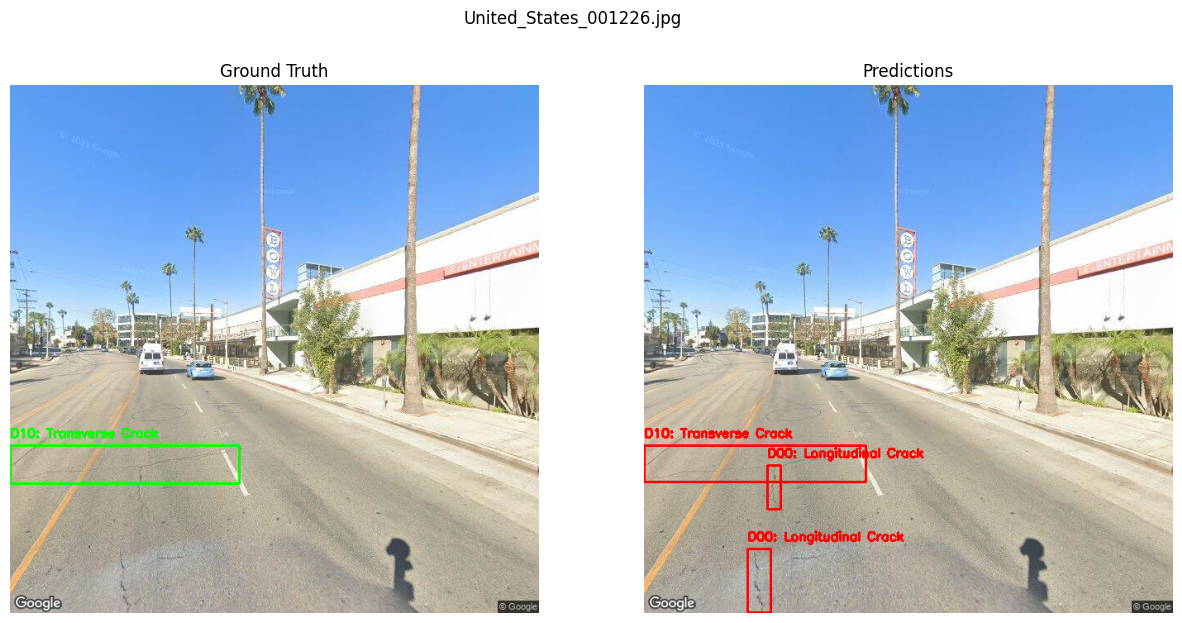
\includegraphics[width=0.6\textwidth]{img/ground_truth_example_1.png}
        \label{fig:ground_truth_example_1}
    }
    \vskip\baselineskip
    \subfigure[Ejemplo en el que el modelo genera varias anotaciones más pequeñas en lugar de una sola grande, como en el \textit{ground truth}.]{
        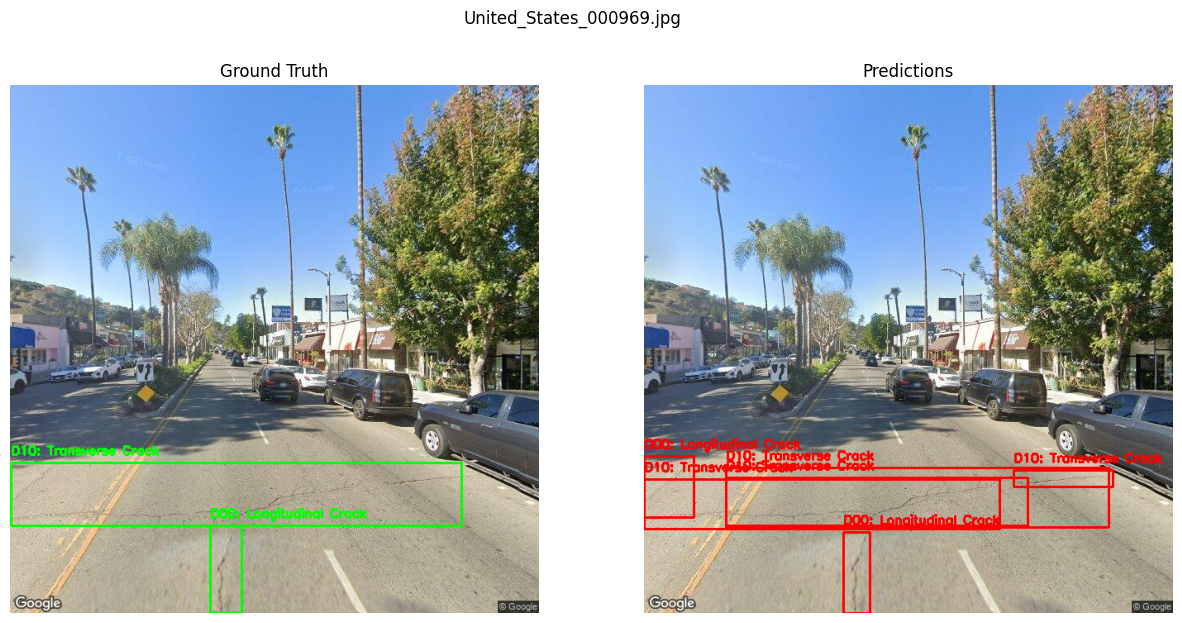
\includegraphics[width=0.6\textwidth]{img/ground_truth_example_4.png}
        \label{fig:ground_truth_example_4}
    }
    \caption{Ejemplos de comparación entre el \textit{ground truth} y las detecciones del modelo.}
    \label{fig:ground_truth_examples}
\end{figure}

% Añadimos la imagen exp1-cv1-confusion_matrix_normalized.png
\begin{figure}[H]
    \centering
    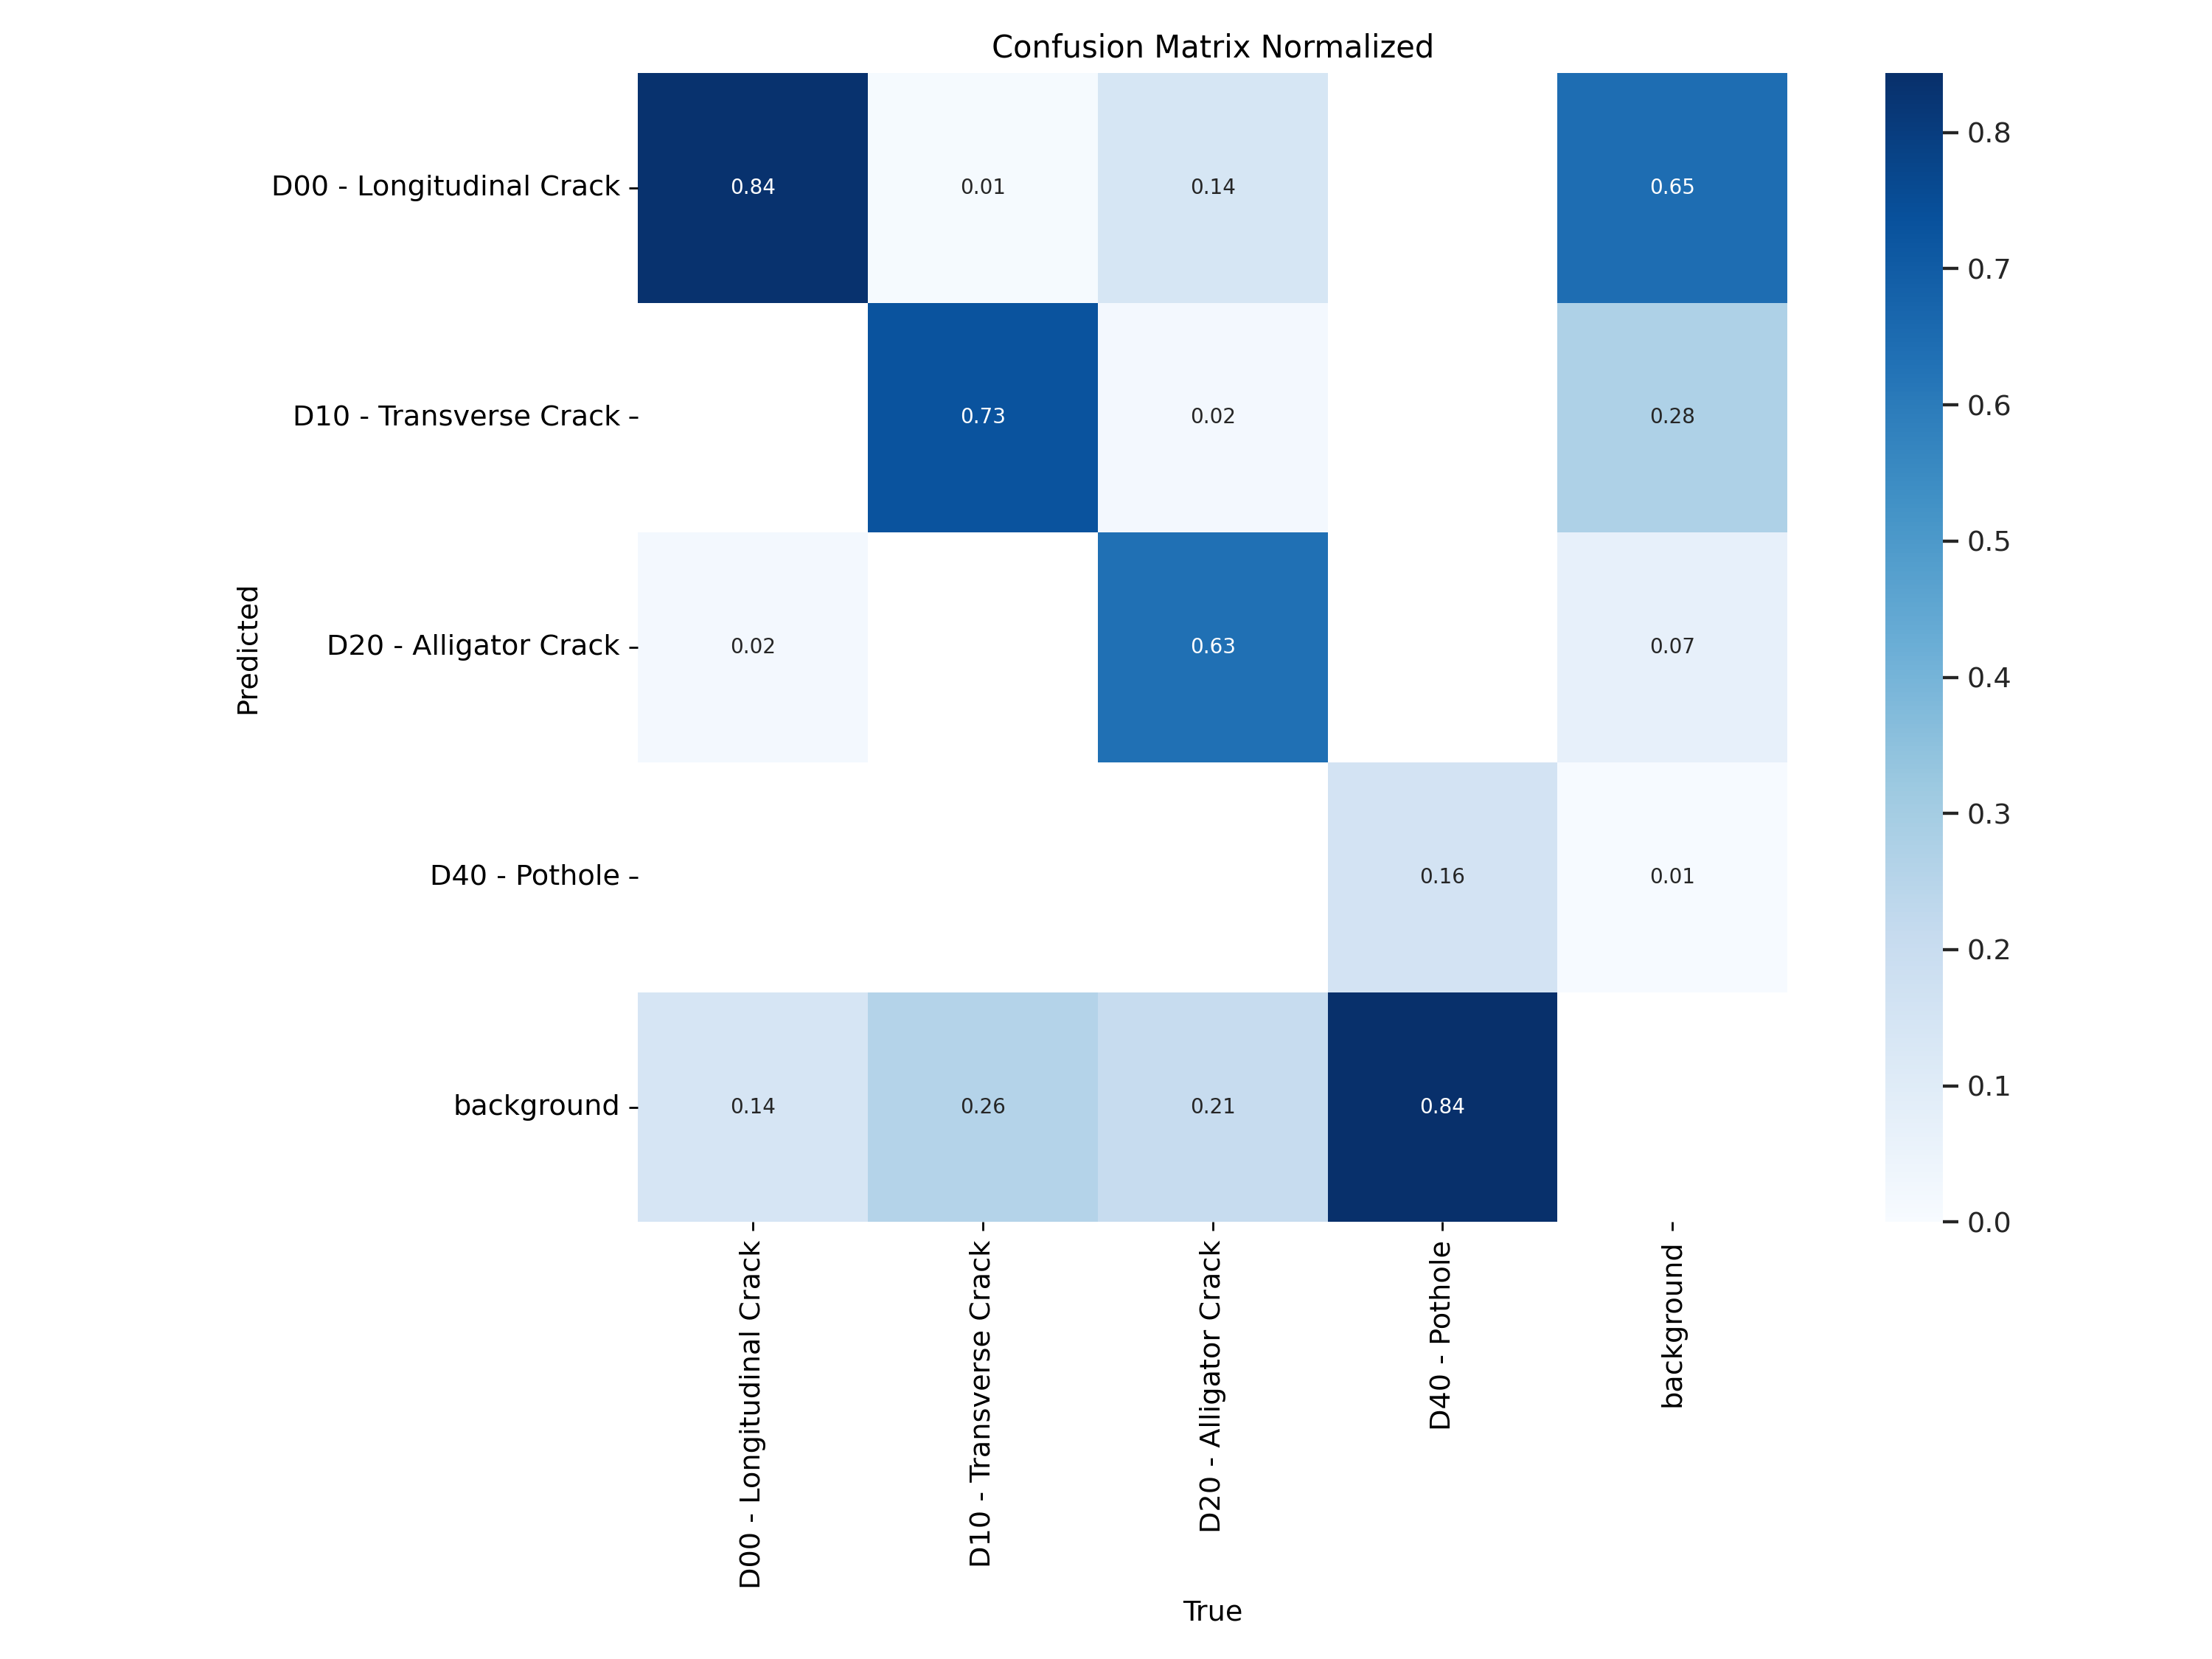
\includegraphics[width=0.6\textwidth]{img/exp1-cv1-confusion_matrix_normalized.png}
    \caption{Matriz de confusión normalizada de la segunda iteración del experimento 1.}
    \label{fig:exp1-cv1-confusion_matrix_normalized}
\end{figure}

\section{Experimento 2: YOLOv8 \textit{very large} con todos los datos de Estados Unidos}\label{SEC:EXP2}

Una forma de mejorar el rendimiento del modelo es aumentar la cantidad de datos de entrenamiento, y otra es incrementar el tamaño del modelo. En este experimento, se busca evaluar cuánto se puede mejorar el rendimiento del modelo entrenado en el experimento 1 al utilizar un modelo YOLOv8 de tamaño \textit{very large} en lugar de \textit{small}, y entrenando con el 100\% de los datos anotados de Estados Unidos en lugar de solo el 75\%. Como se utilizarán todos los datos anotados para entrenar, no se puede confiar en ninguna validación, ya que inevitablemente se utilizarán imágenes vistas durante el entrenamiento para validar. Por lo tanto, en este experimento no se ha realizado validación cruzada.

Se ha utilizado un modelo YOLOv8 de tamaño \textit{very large} y pre entrenado con el conjunto de datos COCO ('yolov8x.pt'). Además, se ha utilizado un tamaño de batch de 15 durante 60 épocas. Estos hiperparámetros se han elegido para ajustarse a las limitaciones de memoria de la GPU Tesla T4 de Google Colab y para que el entrenamiento no dure demasiado tiempo. El entrenamiento ha durado 7 horas. En el anexo \ref{CAP:RES_EXP} se pueden ver el resumen de este entrenamiento generado por Ultralytics.

Una vez entrenado el modelo, se han realizado predicciones para las imágenes de prueba de Estados Unidos y se han subido a la plataforma de la CRDDC2022 para obtener un F1-score sobre los datos de prueba para los que no tenemos \textit{ground truth}. El F1-score obtenido ha sido \textbf{0.607}, lo cual supone una mejora de casi \textbf{18\%} respecto al experimento 1. Debido al aumento del tamaño del modelo, esta mejora en el F1-score tiene asociado un aumento en el tiempo de inferencia. En particular, la inferencia de las 1200 imágenes de prueba de Estados Unidos en un chip Apple M1 Pro ha tardado 2 minutos y 14 segundos para el modelo \textit{small} y 8 minutos y 45 segundos para el modelo \textit{very large}, lo que equivale a \textbf{8.96} imágenes por segundo para el modelo \textit{small} y \textbf{2.29} imágenes por segundo para el modelo \textit{very large}. Esta diferencia en el tiempo de inferencia puede ser un factor crucial a la hora de desplegar el modelo, especialmente si se quiere realizar la inferencia en tiempo real.

Se intentó mejorar el modelo extendiendo el entrenamiento de 60 a 120 épocas. Sin embargo, el F1-score obtenido en la plataforma fue de \textbf{0.604}, casi el mismo que en el experimento 2. Esto sugiere que el modelo ya convergía en 60 épocas o que pierde F1-score debido al sobreajuste con 120 épocas. Dado que se utilizaron todos los datos de entrenamiento, no se puede determinar si el modelo se sobreajustó basándose en los resultados de validación.

Adicionalmente, se realizó un entrenamiento con un YOLOv8 \textit{very large}, utilizando el \textit{fold\_0} como conjunto de validación y el 75\% restante como conjunto de entrenamiento. Este entrenamiento se llevó a cabo durante 150 épocas con un tamaño de batch de 15. El objetivo era determinar cuántas épocas son necesarias para que el modelo \textit{very large} converja y si es posible mejorar el F1-score obtenido en el experimento 2. En las gráficas de 'val/box\_loss' y 'val/dfs\_loss' de la figura \ref{fig:exp2b-results} se observa que, para este entrenamiento con un 75\% de los datos anotados de Estados Unidos, el modelo converge en aproximadamente 90 épocas, después de lo cual comienza a sobreajustar. Como al entrenar con el 100\% de los datos se procesa más información por época, podemos suponer que el modelo converge antes y, por lo tanto, entre 60 y 90 épocas es un rango razonable para entrenar el modelo con el 100\% de los datos.

% Añadir la imagen exp2b-results.png
\begin{figure}[H]
    \centering
    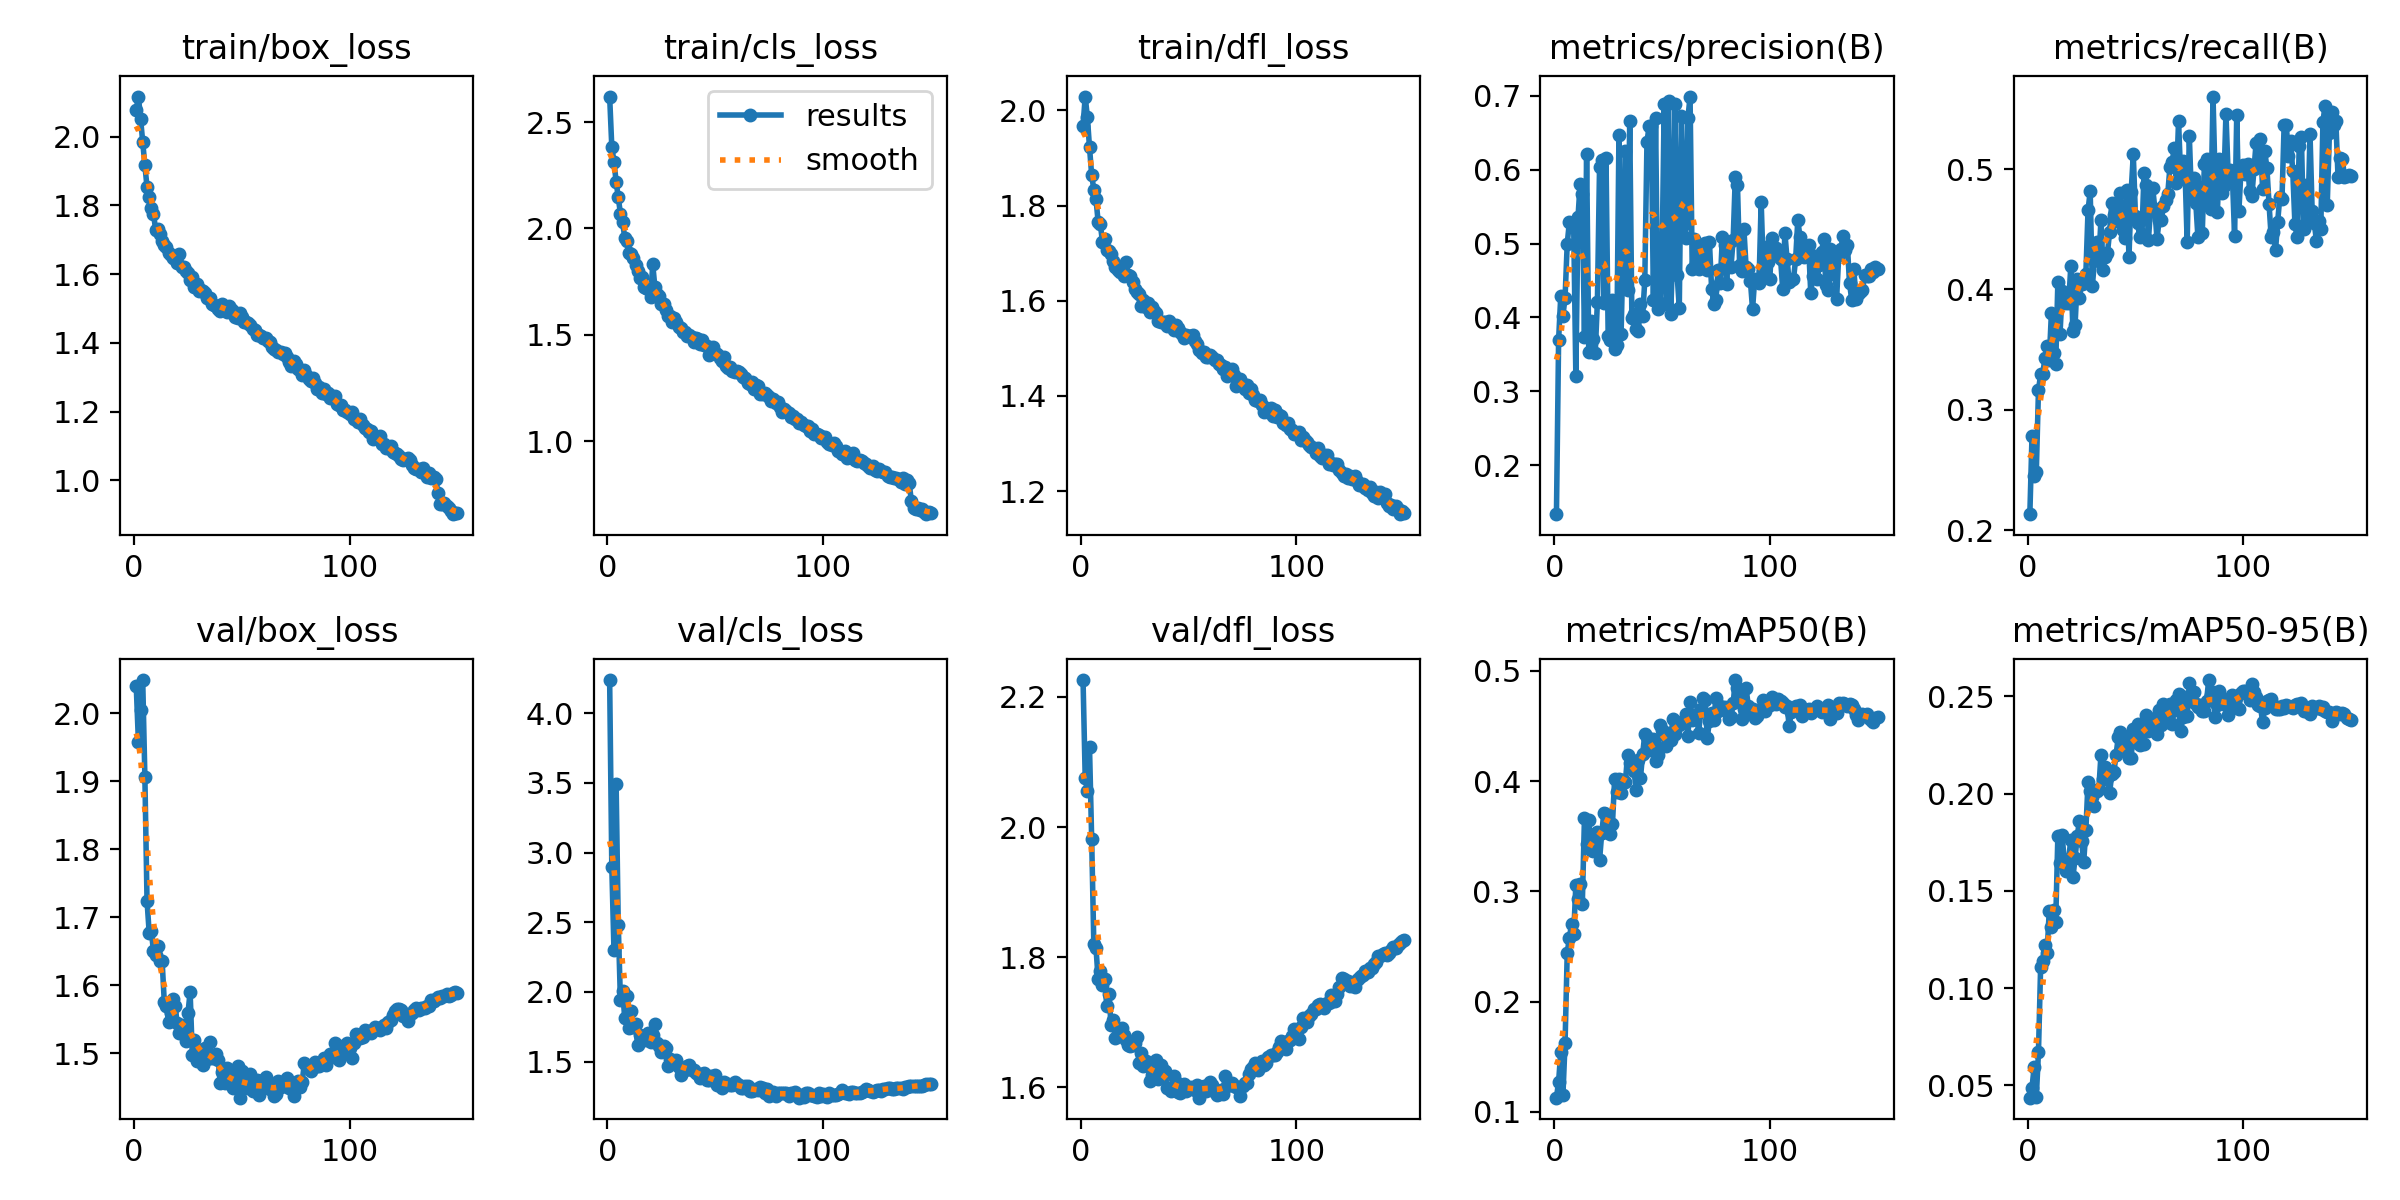
\includegraphics[width=0.9\textwidth]{img/exp2b-results.png}
    \caption{Resultados del entrenamiento del modelo YOLOv8 \textit{very large} con el \textit{fold\_0} como conjunto de validación.}
    \label{fig:exp2b-results}
\end{figure}

En resumen, incrementar el tamaño del modelo de \textit{small} a \textit{very large} y entrenar con todos los datos anotados de Estados Unidos ha mejorado el F1-score del modelo de \textbf{0.515} a \textbf{0.607}, lo que supone una mejora de casi un \textbf{18\%}. Aunque también aumenta el tiempo de inferencia, lo que puede ser un factor crucial a la hora de desplegar el modelo. A partir de este punto, la forma de seguir mejorando el modelo será entrenando con más datos, ya sea de otras regiones o utilizando \textit{data augmentation} para generar más ejemplos de entrenamiento.


\section{Experimento 3: Entrenamiento de modelo base con todos los datos de la CRDDC2022}\label{SEC:EXP3}
En este experimento, se ha entrenado un modelo YOLOv8 de tamaño \textit{very large} con todos los conjuntos de datos de la CRDDC2022. Se ha realizado una validación simple utilizando el 75\% de los datos para entrenamiento y el 25\% para validación (\textit{fold\_0}), sin utilizar validación cruzada debido a la alta demanda computacional de este experimento.

Debido al tamaño del modelo \textit{very large}, el tamaño máximo de batch soportado por las Tesla T4 de Google Colab era de 16. Con 28,784 imágenes de entrenamiento y 9,601 de validación, el batch de 16 resultó en 1,799 iteraciones de entrenamiento y 601 de validación por época. Ejecutando este proceso en Google Colab con una Tesla T4, cada época duraba aproximadamente 43 minutos. El entrenamiento se realizó durante 90 épocas, lo que sumó aproximadamente 65 horas de entrenamiento. Por lo tanto, no era viable realizar una validación cruzada, ya que habría requerido aproximadamente 195 horas adicionales y solo habría garantizado una pequeña mejora en términos de generalización y reducción del riesgo de sobreajuste.

Los pesos de los modelos entrenados en Google Colabs se han descargado y se ha realizado la inferencia en local sobre los distintos conjuntos de datos que componen la CRDDC2022. Los resultados obtenidos en la plataforma de la CRDDC2022 se pueden ver en la tabla \ref{tab:exp3_results}.
\begin{table}[H]
    \centering
    \resizebox{0.35\textwidth}{!}{
        \begin{tabular}{|l|r|}
        \hline
        \textbf{\textit{Leaderboard}} & \textbf{F1-Score} \\ \hline
        Todos           & 0.5969 \\ \hline
        India           & 0.3747 \\ \hline
        Japón           & 0.5946 \\ \hline
        Noruega         & 0.3097 \\ \hline
        Estados Unidos  & 0.6412 \\ \hline
        \textbf{Media}  & 0.5034 \\ \hline
        \end{tabular}
    }
    \caption{F1-scores obtenidos en la plataforma de la CRDDC2022 para los distintos conjuntos de datos.}
    \label{tab:exp3_results}
\end{table}

En el anexo \ref{CAP:LEADERBOARD} se presentan los resultados de los 15 mejores equipos para cada \textit{leaderboard} de la CRDDC2022 al cierre de la competición. Al comparar los resultados de este experimento con los de los mejores equipos de la CRDDC2022, se observa que el modelo entrenado se encuentra ligeramente por debajo del top 15 y lejos de los primeros puestos. Por ejemplo, en el \textit{leaderboard} de todos los datos, el modelo entrenado obtiene un F1-score de \textbf{0.597}, mientras que los 15 mejores equipos obtuvieron entre 0.605 y 0.770. Es decir, aunque el modelo entrenado casi entra en el top 15, queda muy lejos del primer puesto. Por otro lado, la inferencia se ha realizado en un chip Apple M1 Pro y ha tardado 77 minutos y 2 segundos para las 9035 imágenes de test, lo que corresponde a \textbf{1.95} imágenes por segundo. 

El tiempo de inferencia es muy alto y limitaría la capacidad de despliegue de este modelo en un entorno de producción que requiera inferencia en tiempo real. Algunas soluciones en términos de despliegue serian utilizar un tamaño de modelo más pequeño, procesar las imágenes en \textit{off-line} desde un servidor central o limitar la velocidad de los vehículos que recogen las imágenes para reducir el requisito de imágenes por segundo. En cualquier caso, este problema es común en las soluciones propuestas por los equipos de la CRDDC2022, por lo que una posible línea de trabajo futuro sería optimizar el modelo para reducir el tiempo de inferencia, de hecho, la nueva edición de la RDDC, la ORDDC2024 \cite{ORDDC2024}, tiene como principal objetivo la optimización de los modelos para reducir el tiempo de inferencia y uso de recursos (ver sección \ref{SEC:TRABFUT}).

Es importante recordar que en este trabajo se ha utilizado YOLOv8 en lugar de YOLOv7 y YOLOv5, que eran las versiones disponibles durante la CRDDC2022, ya que YOLOv8 aún no existía en ese momento. Sin embargo, la mayoría de los equipos participantes emplearon \textit{ensembles} de varios modelos y otras técnicas avanzadas que les permitieron obtener mejores puntuaciones, incluso utilizando una versión anterior de YOLO. Esto sugiere que nuestro sistema base tiene un amplio margen de mejora si se aplican técnicas similares, especialmente \textit{ensembles} de modelos. El objetivo de este TFG era desarrollar un sistema base basado en YOLOv8, al que posteriormente se le puedan aplicar algunas de estas técnicas. En la sección \ref{SEC:TRABFUT} se proponen algunas líneas de trabajo futuro para mejorar el rendimiento del modelo.

Otra consideración sobre este modelo es que no se han utilizado todos los datos anotados para entrenar, ya que se ha reservado un 25\% de los datos para la validación. Es probable que entrenando con todos los datos, sin reservar una porción para validación, se puedan obtener resultados ligeramente mejores. Sin embargo, debido a las limitaciones computacionales y de tiempo, no se ha realizado dicho entrenamiento.

En general, una estrategia que se podría seguir en estos casos es realizar primero una validación con un subconjunto de los datos para determinar el número de épocas necesarias para que el modelo converja. Posteriormente, se podría entrenar el modelo con todos los datos y sin validación, durante el número de épocas determinado anteriormente. Esta estrategia no garantiza que el modelo no se sobreajuste en ausencia de validación, pero podría ayudar a aprovechar al máximo los datos disponibles para el entrenamiento.

A continuación, analizaremos los resultados obtenidos en la plataforma (ver tabla \ref{tab:exp3_results}) junto con resultado de la validación sobre el \textit{fold\_0} para entender mejor las limitaciones del modelo y posibles áreas de mejora. El anexo \ref{CAP:RES_EXP} contiene los resultados completos de la validación de este experimento y las matrices de confusión para todos los datos y desglosadas por región. 

En los \textit{leaderboards} de India y Noruega se han obtenido resultados significativamente peores que en otros conjuntos de datos. Esto no es un problema exclusivo de nuestro modelo, ya que los participantes de la CRDDC2022 también experimentaron dificultades similares. No obstante, esto indica que estos conjuntos de datos presentan desafíos adicionales que deben considerarse.

En el caso de India, la calidad de las imágenes es la más baja de todos los conjuntos de datos (ver figura \ref{fig:example_images_region}), y la distribución de los tipos de daño es muy diferente, con una proporción significativamente alta de grietas de cocodrilo y baches (ver tabla \ref{tab:anotaciones_por_clase_region}). El hecho de que el entrenamiento se realice con una distribución de clases diferente a la de validación puede ser una de las causas de los malos resultados en India.

En el caso de Noruega, las imágenes tienen una resolución muy alta y el pavimento suele ocupar un porcentaje pequeño de la imagen (ver figura \ref{fig:example_images_region}). Estos dos factores hacen que, al redimensionar las imágenes durante el entrenamiento, el número de píxeles dedicados al pavimento sea muy pequeño, impidiendo así la detección de daños pequeños. Al observar las matrices de confusión de Noruega (ver figuras \ref{fig:exp3_val0_norway_confusion_matrix_normalized} y \ref{fig:exp3_val0_norway_confusion_matrix}), se puede ver que el modelo no consigue detectar la mayoría de los daños, lo que indica que el problema no radica en la existencia de muchos falsos positivos, sino en la incapacidad del modelo para detectar daños reales debido al pequeño tamaño de los píxeles dedicados al pavimento. En la figura \ref{fig:CRDDC2022_detailed_solutions}, se observa que una de las características de la solución del tercer equipo, MDPT, fue recortar las imágenes de Noruega para centrarse en el pavimento. Esta es una estrategia que podría probarse. No obstante, esta solución limita la generalización, ya que se trata de una actuación \textit{ad-hoc} focalizada en mejorar el rendimiento en un conjunto de datos específico. La alternativa para generalizar sería crear un algoritmo que detecte pavimentos y recorte las imágenes automáticamente, lo cual es una tarea más compleja que la propuesta por MDPT.

Las particularidades de estos dos conjuntos de datos podrían capturarse mediante un \textit{ensemble} de modelos que incluyan modelos específicamente entrenados para tener en cuenta estas características específicas de las imágenes de India y Noruega.

En la figura \ref{fig:exp3-val0-all-confusion_matrix_normalized} se puede ver la matriz de confusión normalizada del modelo entrenado en el experimento 3 sobre todos los datos de validación. Se observa que el modelo genera muchos falsos positivos especialmente de grietas longitudinales. Como se comentó en experimentos anteriores muchas de estas predicciones son correctas, pero no aparecen en el \textit{ground truth}. De cara a obtener un mejor F1-score en la competición se deberían de buscar soluciones a este problema como algoritmos de post-procesado que puedan descartar o fusionar predicciones para adaptarse mejor al \textit{ground truth}. Por otro lado, al igual que en experimentos anteriores, los baches son el tipo de daño que peor detecta el modelo, esto puede deberse a que es el tipo de daño con el menor número de anotaciones y por lo tanto el modelo no generaliza bien en este tipo de daño. Puede ser interesante explorar técnicas de \textit{data augmentation} para generar más ejemplos de baches o añadir al entrenamiento un conjunto de datos especifico de baches.

En las figuras \ref{fig:exp3-val-all-curves} se pueden ver las curvas de F1-score en función del umbral y precisión vs \textit{recall} para el modelo entrenado en el experimento 3 sobre el \textit{fold\_0} de todos los datos de validación. Se observa que el umbral óptimo para el modelo es aproximadamente 0.3, lo cual es parecido al umbral por defecto de 0.25 que hemos usado con Ultralytics. Adicionalmente, en ambas gráficas vemos que los peores resultados vienen de los baches, mientras que los mejores vienen de las grietas de cocodrilo. Esto es consistente con lo que hemos visto previamente y refuerza la necesidad de buscar soluciones específicas para los baches.

En resumen, el tercer experimento consistió en entrenar un modelo YOLOv8 de tamaño \textit{very large} utilizando todos los conjuntos de datos de la CRDDC2022. Se ha obtenido un F1-score global de \textbf{0.597}, lo que indica que el modelo es capaz de generalizar en una variedad de conjuntos de datos y puede resultar útil como base para futuros trabajos de detección de daños en pavimentos. Además, se han identificado las limitaciones del modelo y posibles áreas de mejora. En la sección \ref{SEC:TRABFUT} se proponen algunas líneas de trabajo futuro para expandir el modelo base y mejorar su rendimiento.

% Añadimos la imagen exp3-val0-all-confusion_matrix_normalized.png
\begin{figure}[H]
    \centering
    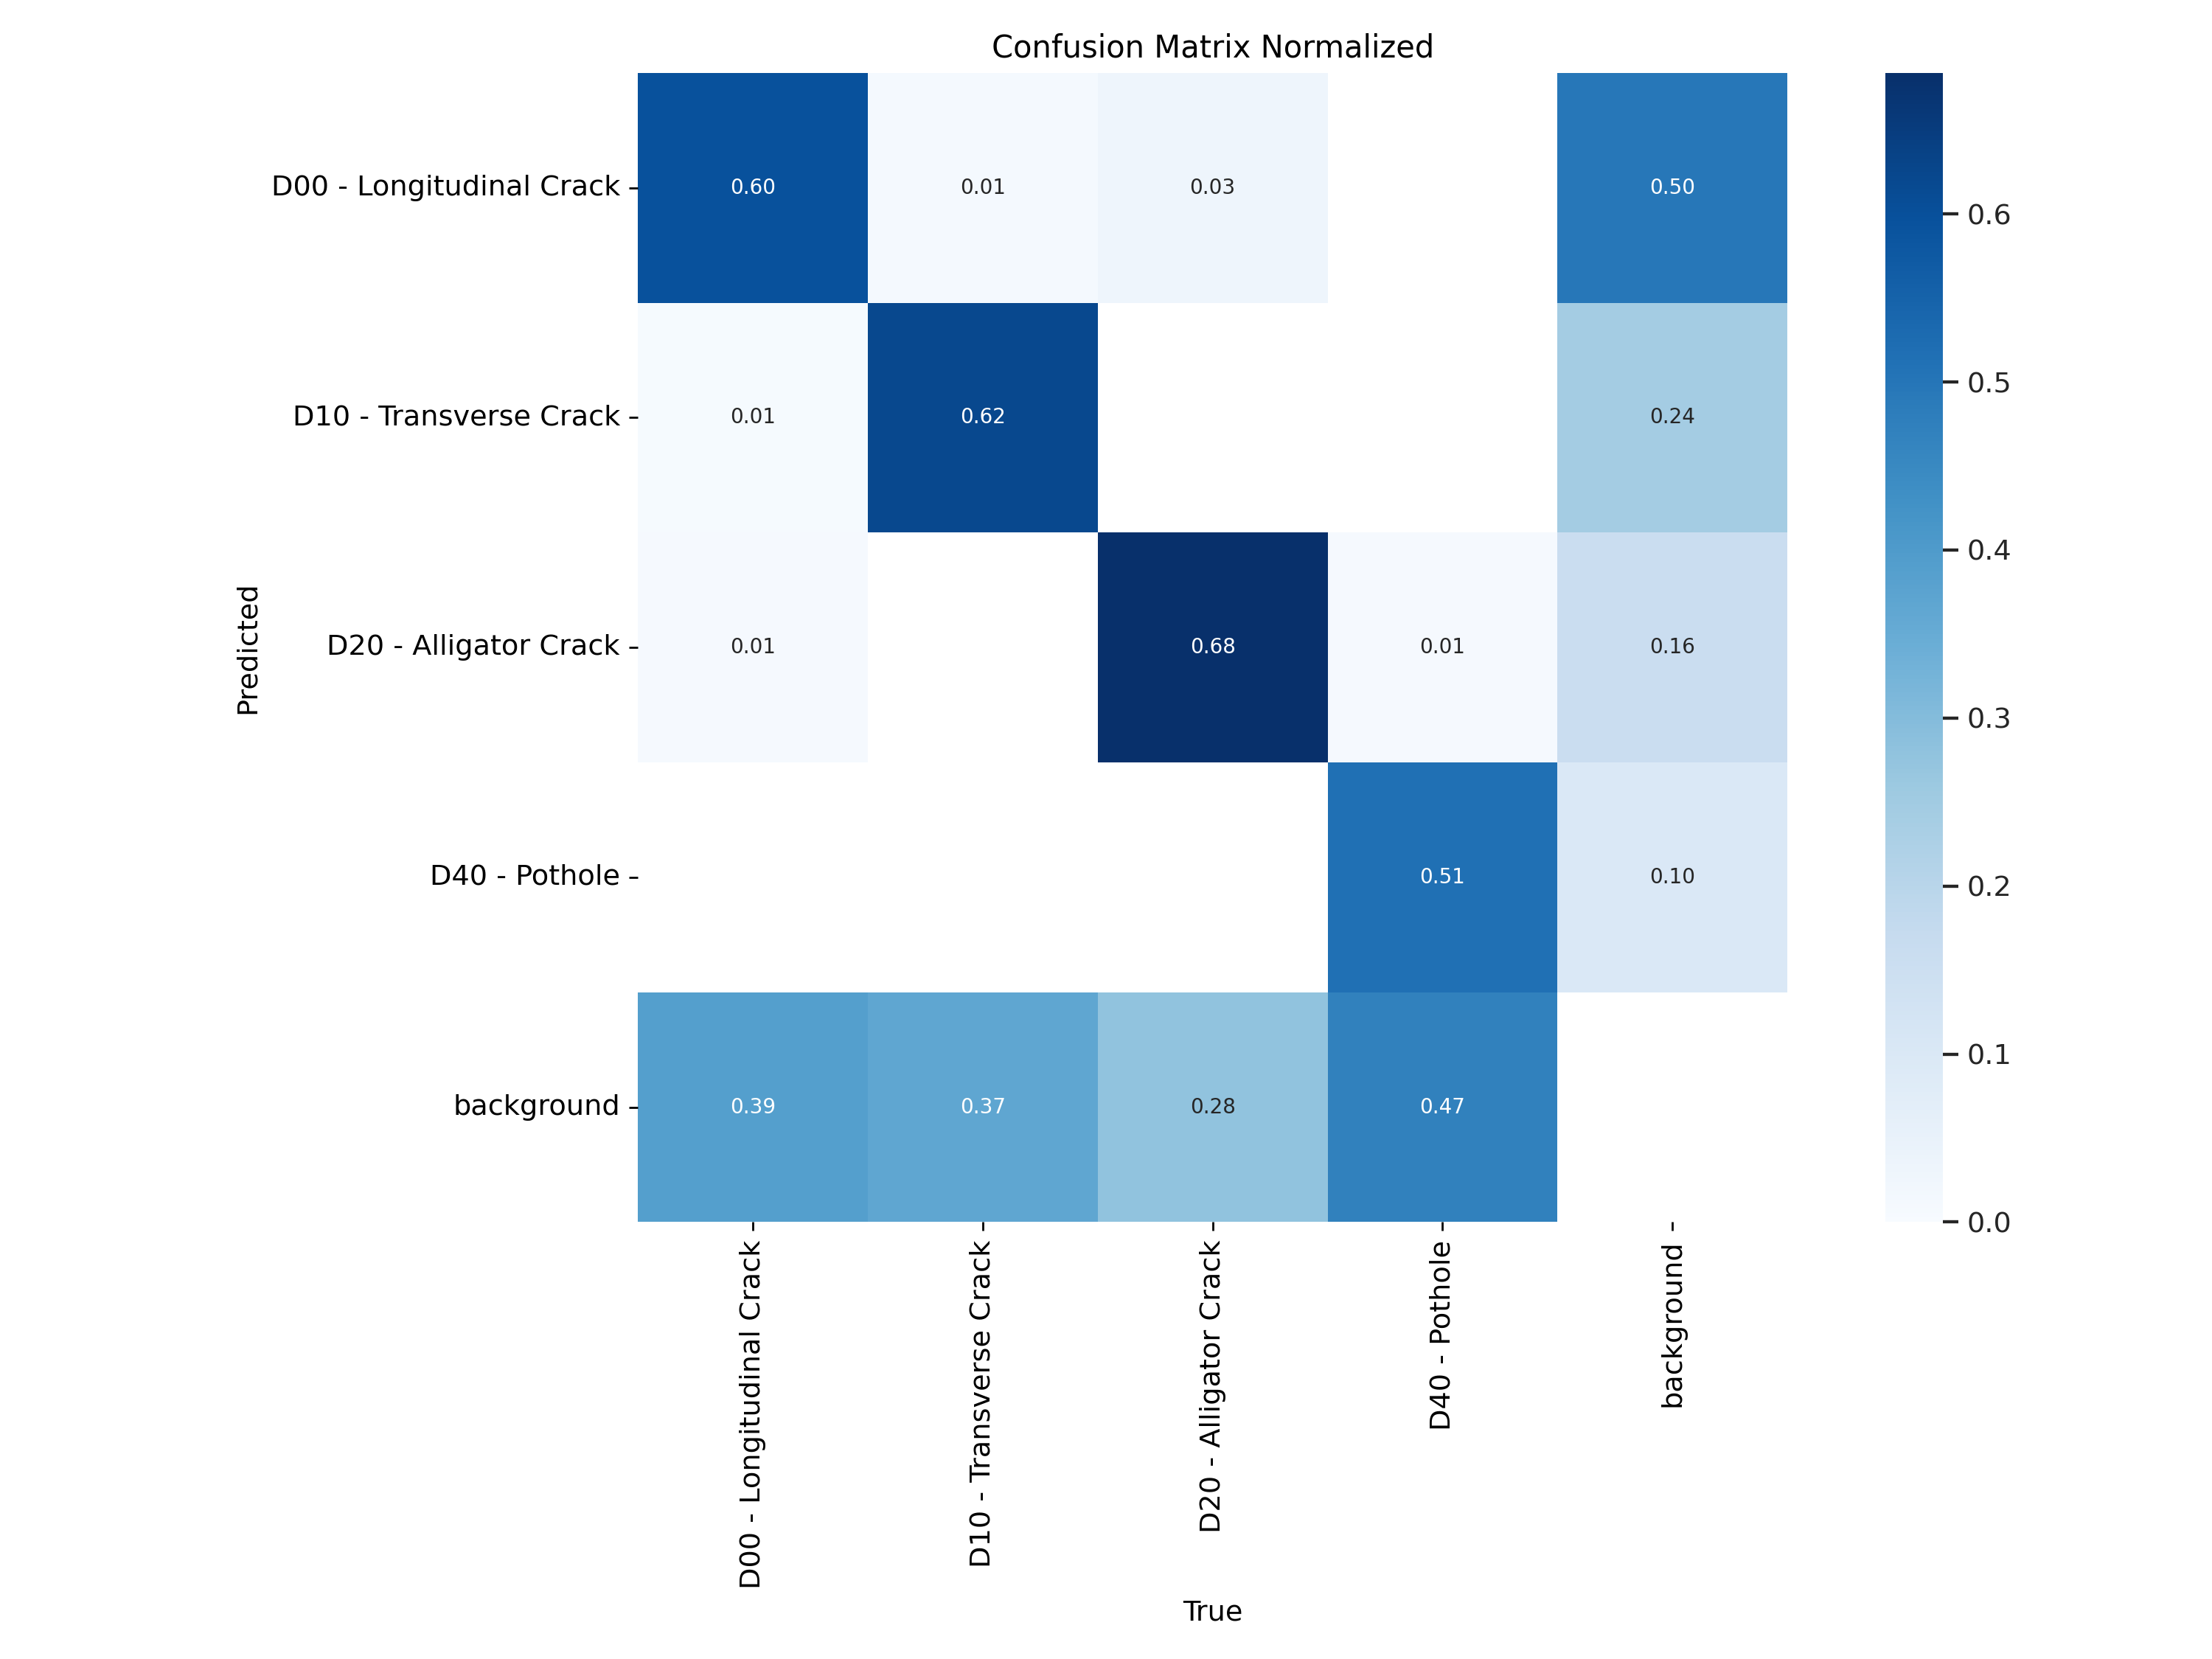
\includegraphics[width=0.9\textwidth]{img/exp3-val0-all-confusion_matrix_normalized.png}
    \caption{Matriz de confusión normalizada del modelo entrenado en el experimento 3 sobre el \textit{fold\_0} de todos los datos de validación.}
    \label{fig:exp3-val0-all-confusion_matrix_normalized}
\end{figure}

% Anadimos la imagen exp3-val-all-F1_curve.png y exp3-val-all-PR_curve.png
\begin{figure}[H]
    \centering
    \subfigure[F1-score en función del umbral.]{
        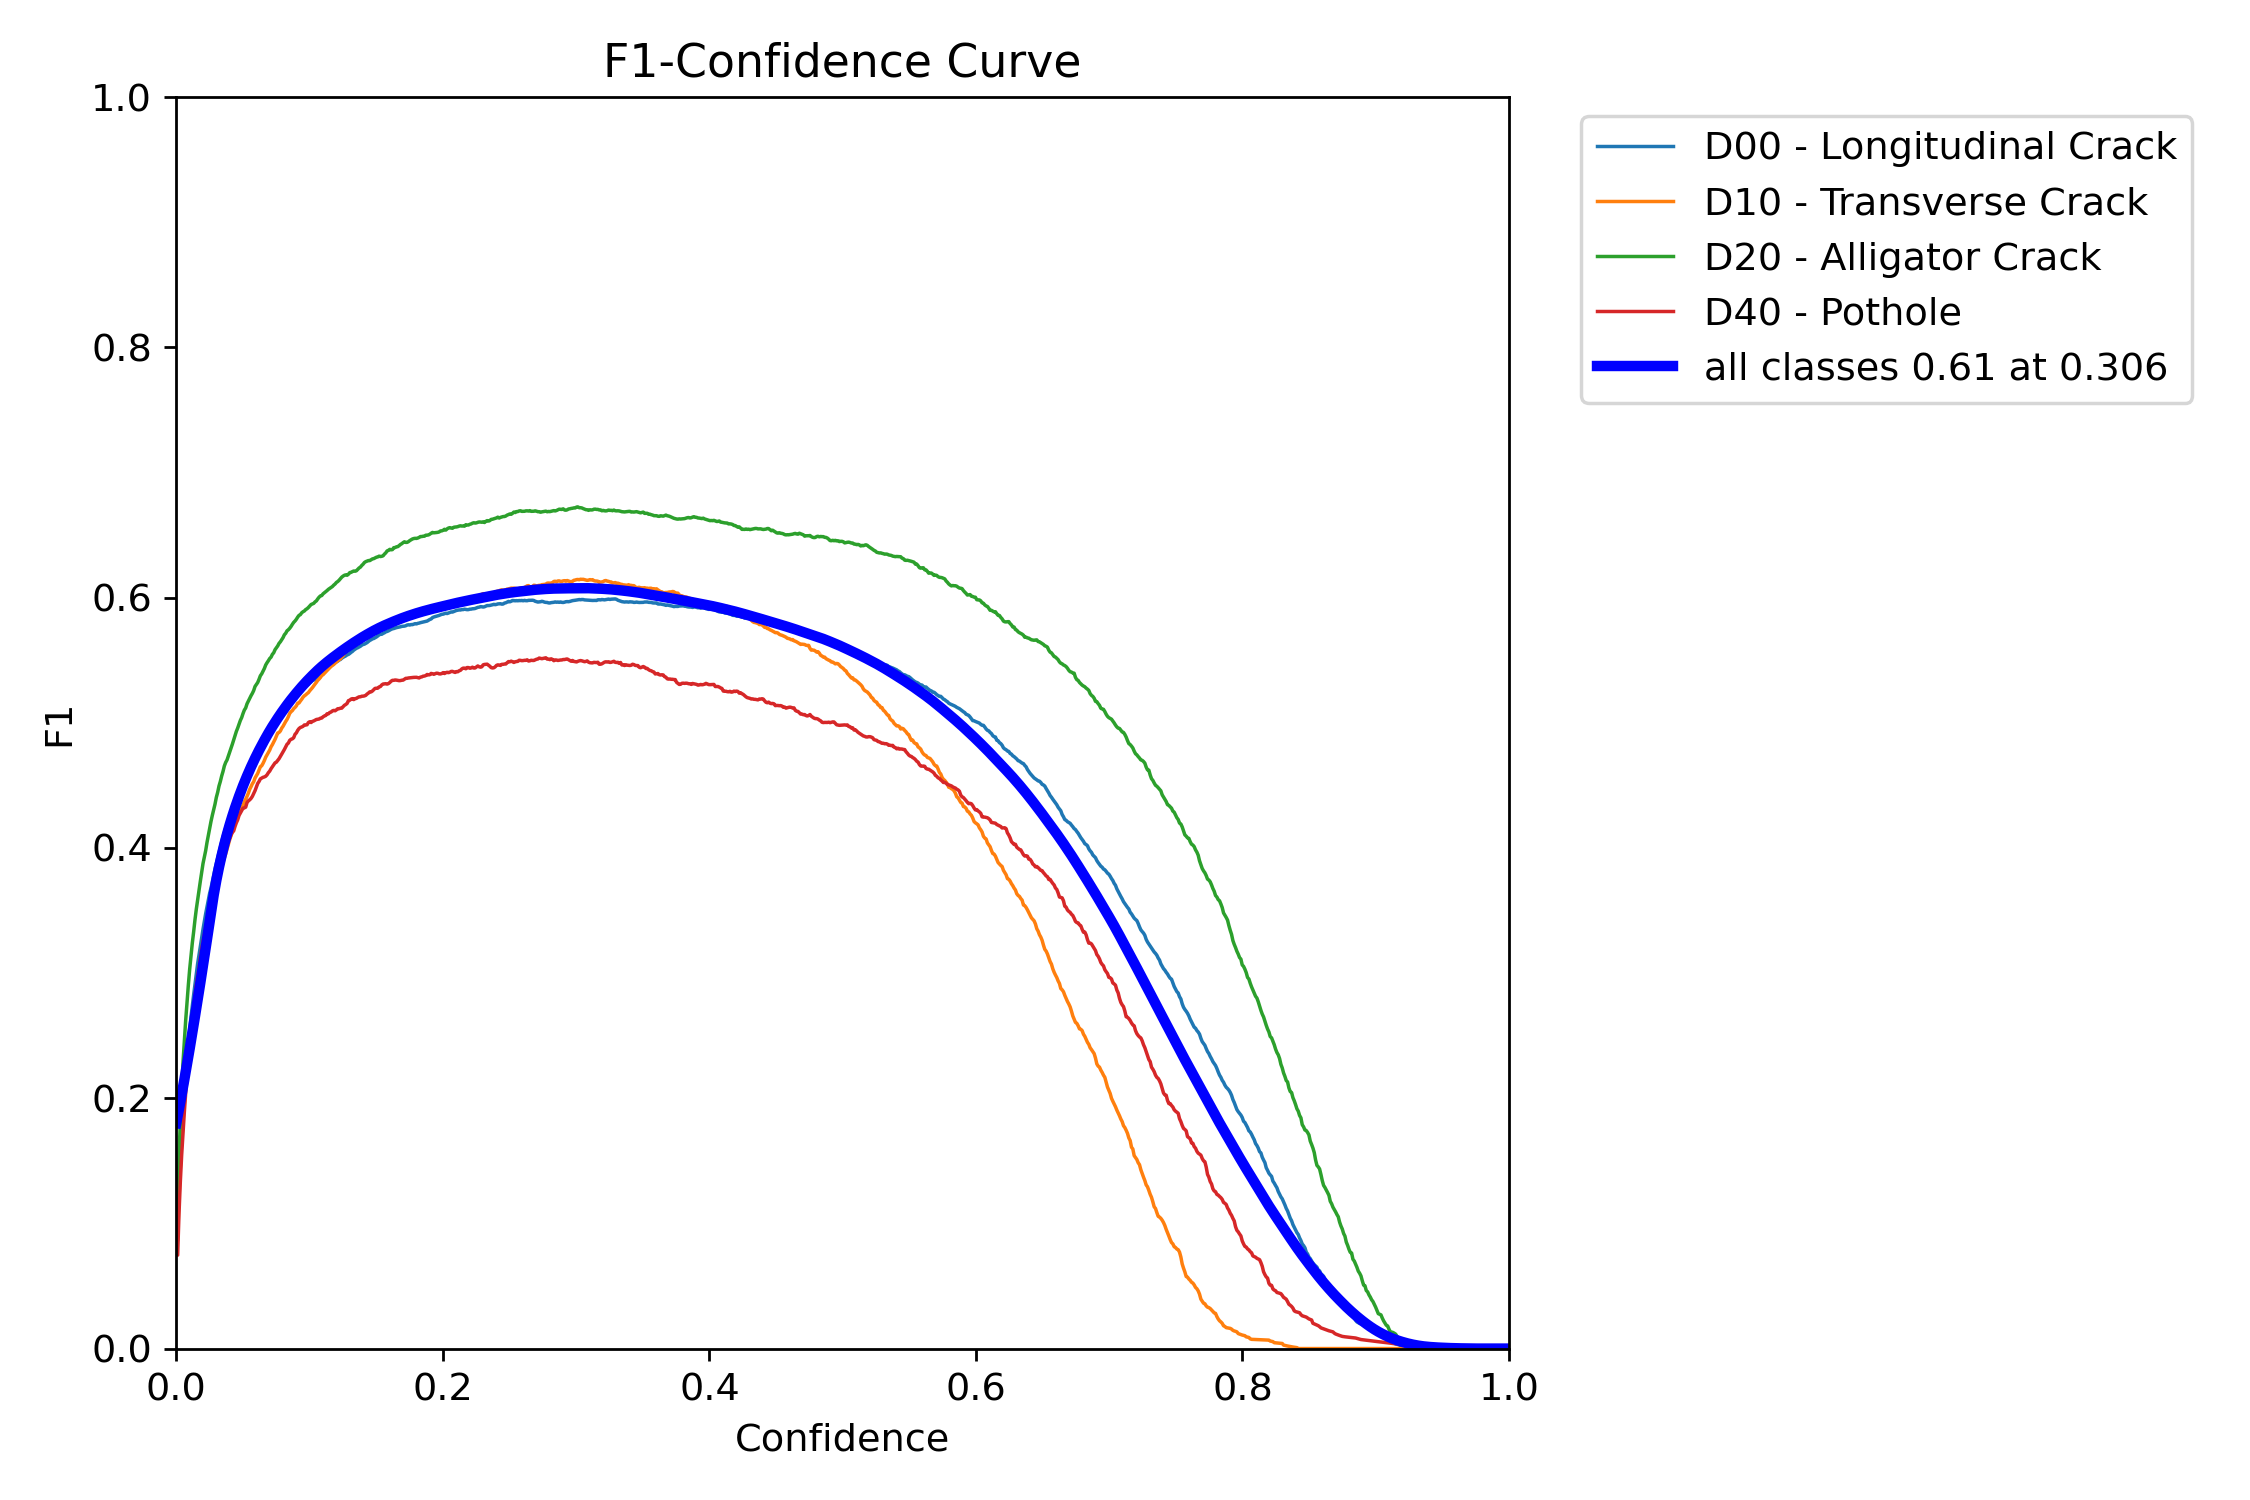
\includegraphics[width=0.45\textwidth]{img/exp3-val-all-F1_curve.png}
        \label{fig:exp3-val-all-F1_curve}
    }
    \subfigure[Precisión vs \textit{recall}.]{
        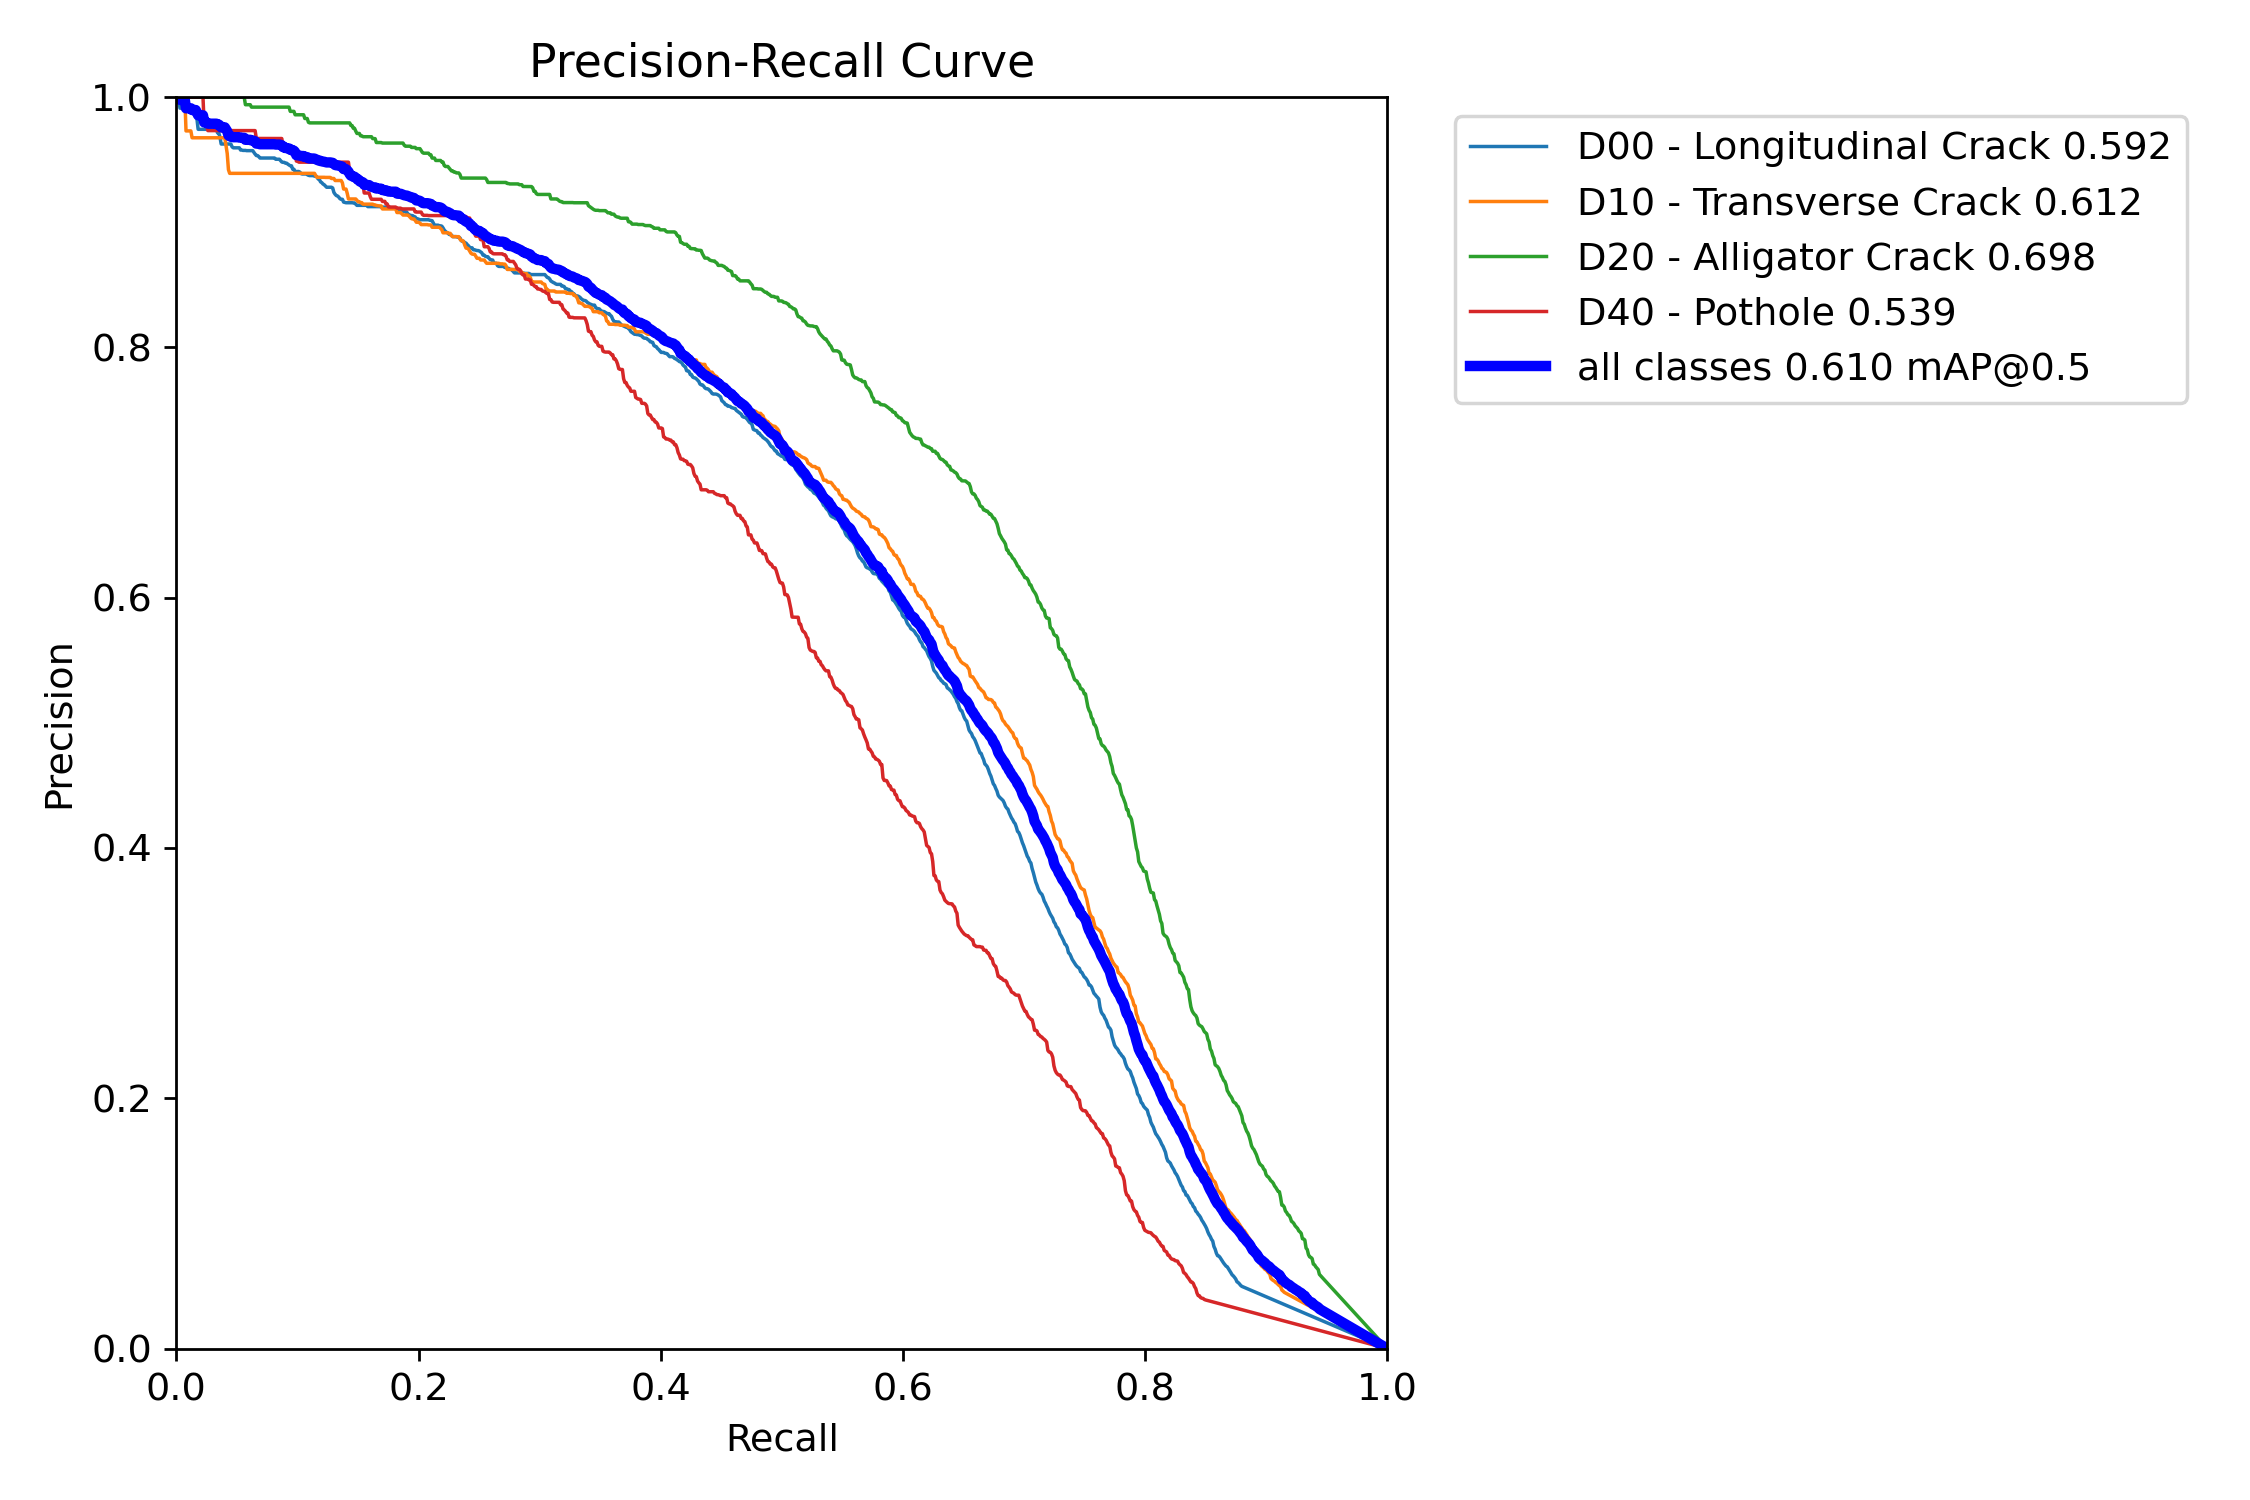
\includegraphics[width=0.45\textwidth]{img/exp3-val-all-PR_curve.png}
        \label{fig:exp3-val-all-PR_curve}
    }
    \caption{Curvas de F1-score en función del umbral y precisión vs \textit{recall} para el modelo entrenado en el experimento 3 sobre el \textit{fold\_0} de todos los datos de validación.}
    \label{fig:exp3-val-all-curves}
\end{figure}